\chapter{COCOMO II Approach} \label{chap3}
For carrying out this section of the document we are referring to the COCOMO II model definition manual at:\\
\href{http://csse.usc.edu/csse/research/COCOMOII/cocomo2000.0/CII\_modelman2000.0.pdf}{http://csse.usc.edu/csse/research/COCOMOII/cocomo2000.0/CII\_modelman\\2000.0.pdf}.\\
Following this document we have compiled the two tables below, and then we have used the online calculator at this web page: \href{http://csse.usc.edu/tools/COCOMOII.php}{http://csse.usc.edu/tools/\\COCOMOII.php} to compute the effort, the total cost, the duration and the number of person estimated for the completion of the project.

\begin{table}[!htbp]
\begin{center}
\begin{tabular}[t]{|p{0.3\textwidth}|p{0.15\textwidth}|c|}
\hline
\textbf{Scale Driver} & \textbf{Factor} & \textbf{Value} \\
\hline
\hline
Precedentedness & Very Low & 6,20 \\
\hline
Development Flexibility & Nominal & 3,04 \\
\hline
Risk Resolution & Low & 5,65 \\
\hline
Team Cohesion & Extra High & 0 \\
\hline
Process Maturity & High & 3,12 \\
\hline
\end{tabular}
\end{center}
\end{table}
\clearpage

\begin{table}[!htbp]
\begin{center}
\begin{tabular}[t]{|p{0.55\textwidth}|p{0.15\textwidth}|c|}
\hline
\textbf{Cost Driver} & \textbf{Factor} & \textbf{Value} \\
\hline
\hline
Required Software Reliability & Nominal & 1 \\
\hline
Data Base Size & Nominal & 1 \\
\hline
Product Complexity & Nominal & 1 \\
\hline
Required Reusability & High & 1,07 \\
\hline
Documentation match to life-cycle needs & High & 1 \\
\hline
Execution Time Constraint & Nominal & 1 \\
\hline
Main Storage Constraint & Nominal & 1 \\
\hline
Platform Volatility & Nominal & 1 \\
\hline
Analyst Capability & Low & 1,19 \\
\hline
Programmer Capability & Nominal & 1 \\
\hline
Application Experience & Low & 1,10 \\
\hline
Platform Experience & Low & 1,09 \\
\hline
Language and Tool Experience & Nominal & 1 \\
\hline
Personnel Continuity & Very Low & 1,29 \\
\hline
Usage of Software Tools & Nominal & 1 \\
\hline
Multisite development & Low & 0,86 \\
\hline
Required Development Schedule & Nominal & 1 \\
\hline
\end{tabular}
\end{center}
\end{table}

\begin{figure}[!htbp]
\centering
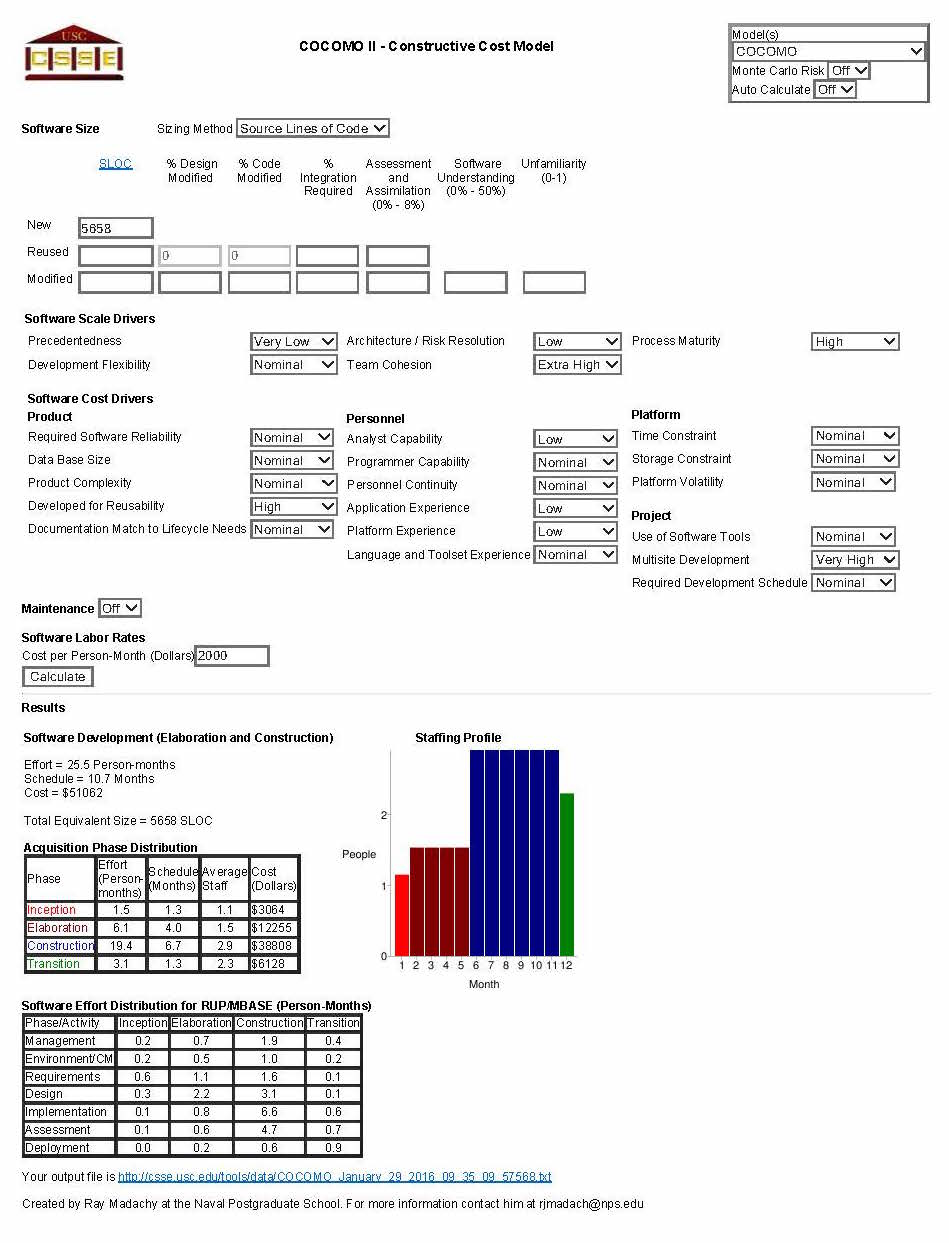
\includegraphics[width=\textwidth]{cpt/img/COCOMOII-ConstructiveCostModel}
\caption{Representation of effort, total cost, duration and number of person estimated for the completion of the project.}
\end{figure}

\noindent So, in conclusion we have found these values for effort, total cost, duration and members of the project:\\
\textbf{Effort} = 25,5 Person-Months \\
\textbf{Cost} (assuming an average cost per Person-Month of 2.000,00 \$) = 51.062,00 \$ \\
\textbf{Duration} = 10,7 months \\
\textbf{Team size} = $25,5 / 10,7 = 2,38$ members \\